%\section*{List of Figures}
\begin{figure}[b]
    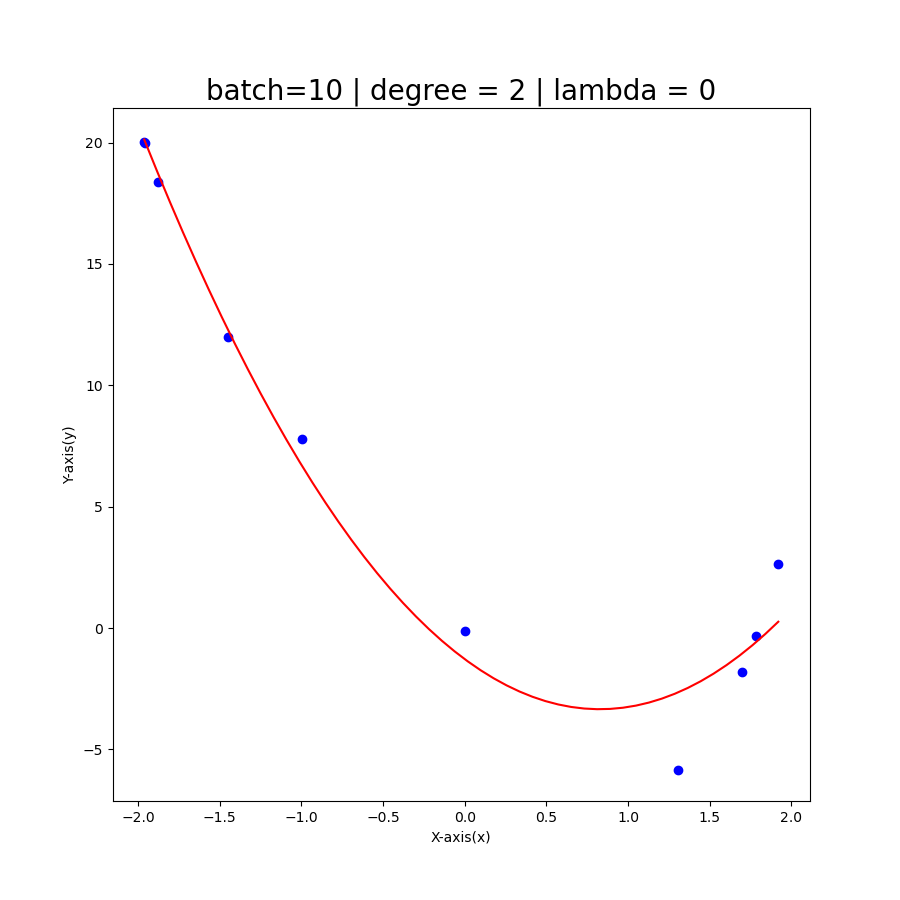
\includegraphics[width=.24\textwidth]{Task 1 Images/Batch 10/Figure_1.png}\hfill
    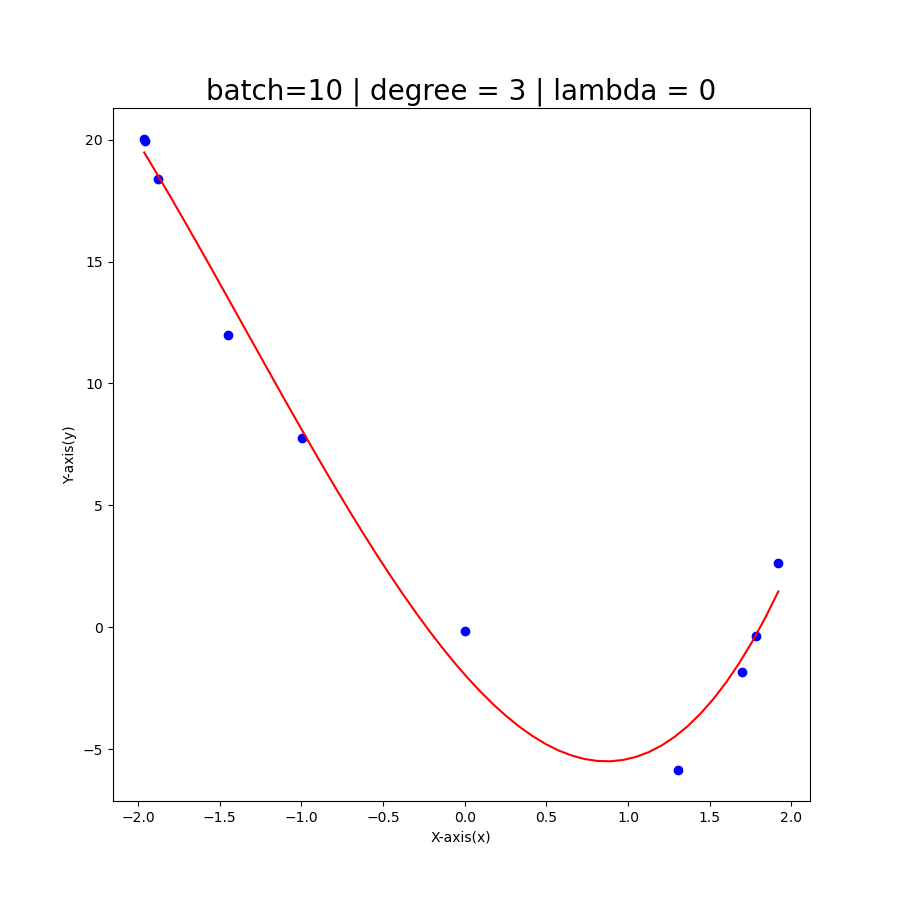
\includegraphics[width=.24\textwidth]{Task 1 Images/Batch 10/Figure_2.png}\hfill
    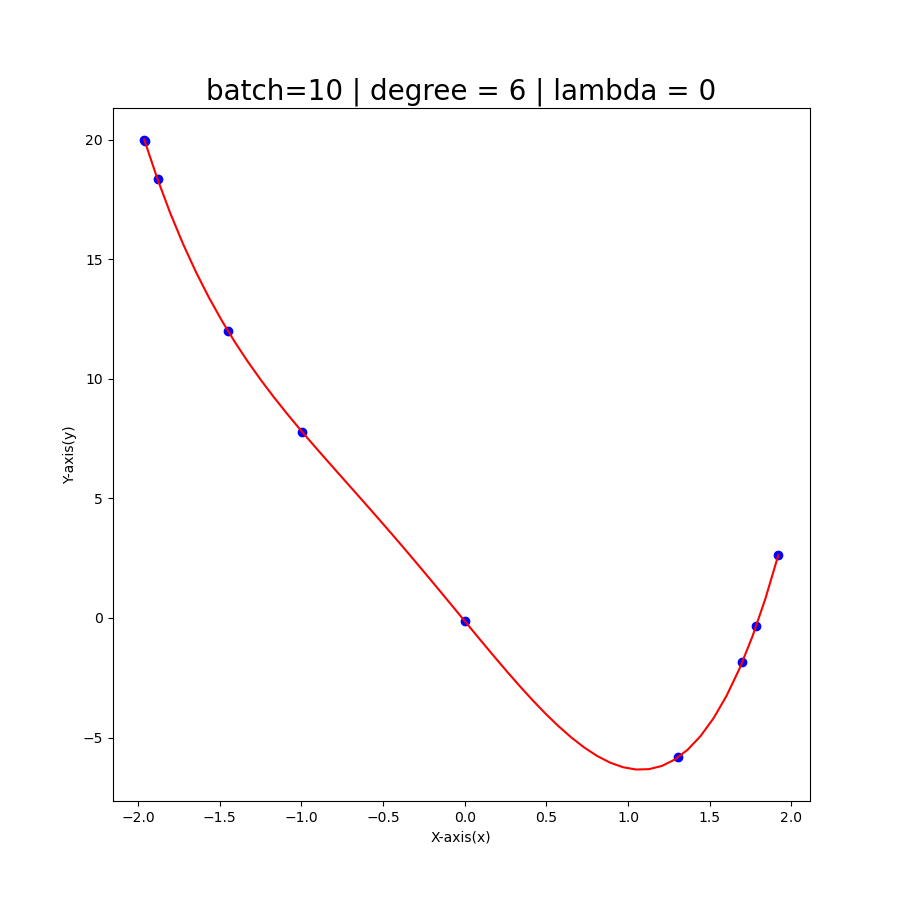
\includegraphics[width=.24\textwidth]{Task 1 Images/Batch 10/Figure_3.png}\hfill
    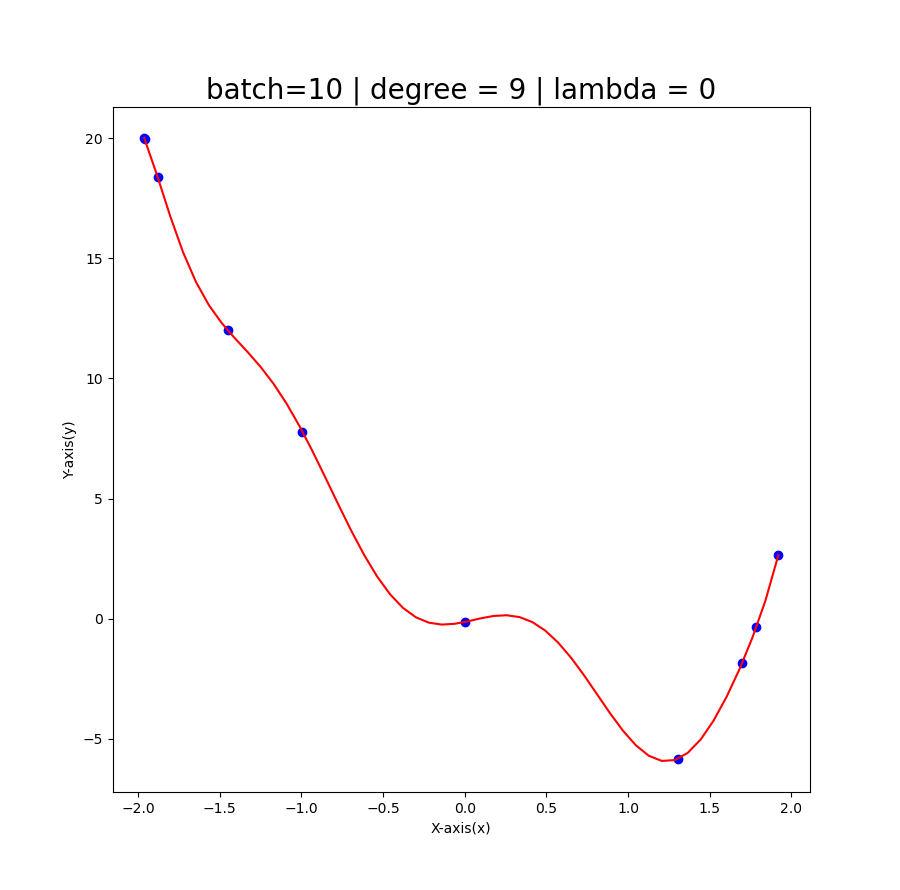
\includegraphics[width=.24\textwidth]{Task 1 Images/Batch 10/Figure_4.png}
    \caption{Plots of Polynomials having various orders of degree for a fixed regularistion parameter $\lambda = 0$ using 10 samples}
    \label{fig:1}
    \vspace*{\floatsep}

    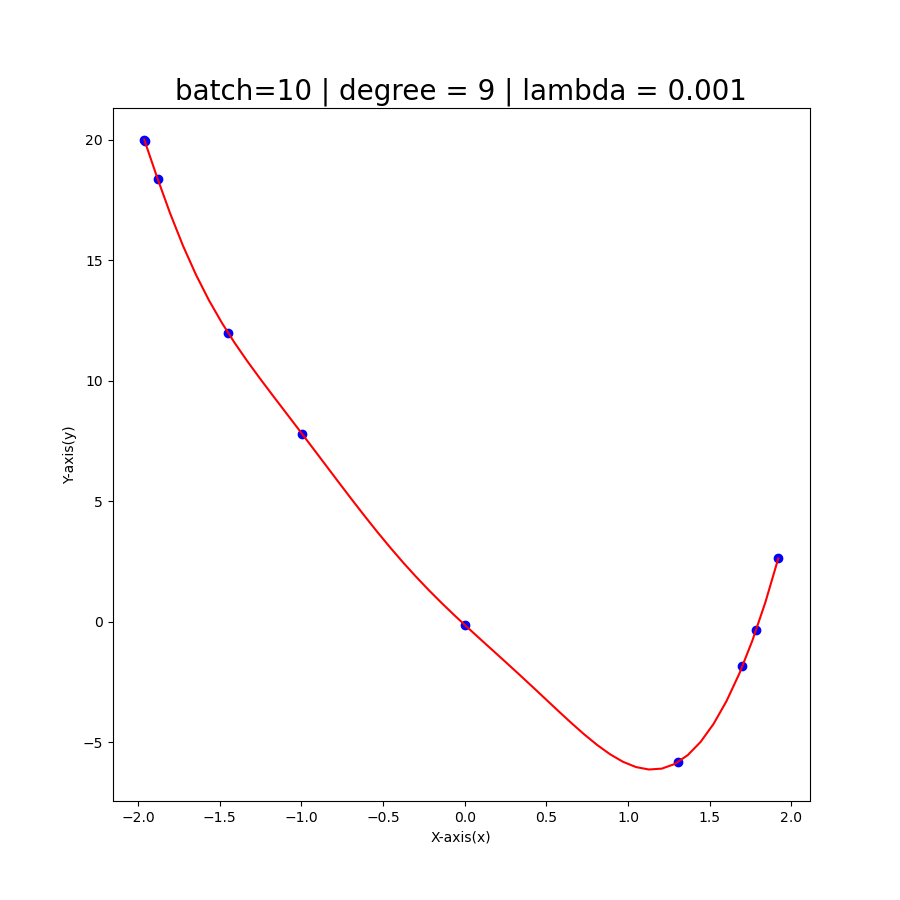
\includegraphics[width=.24\textwidth]{Task 1 Images/Batch 10/Figure_5.png}\hfill
    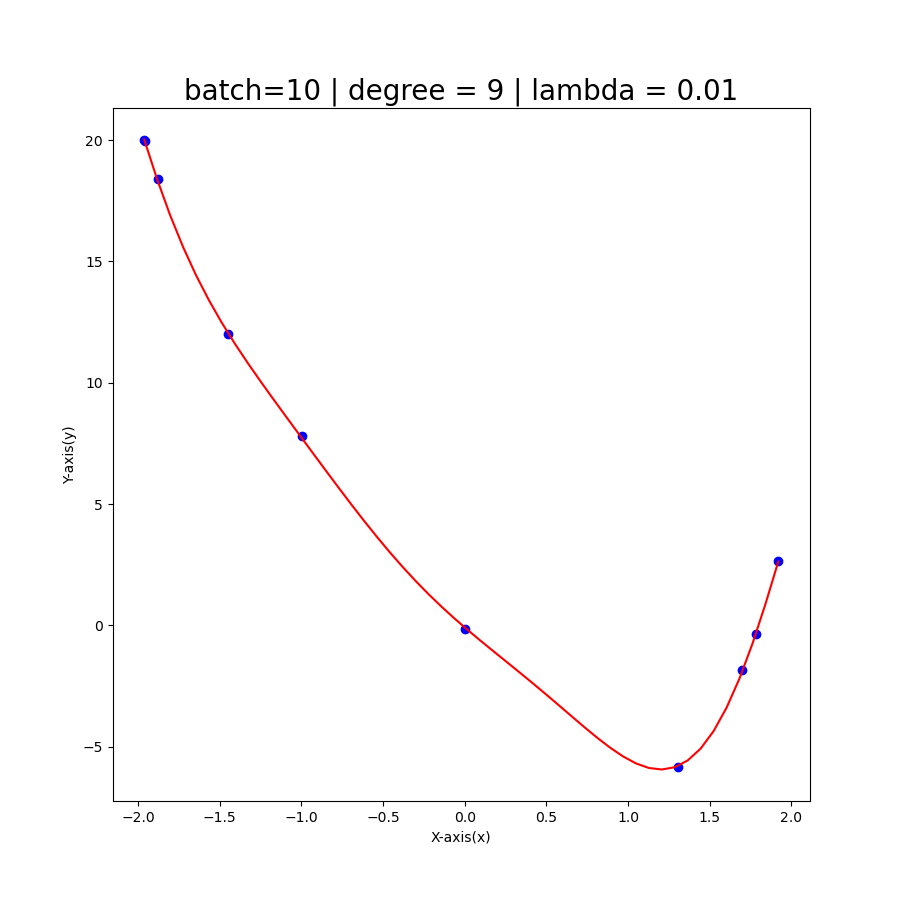
\includegraphics[width=.24\textwidth]{Task 1 Images/Batch 10/Figure_6.png}\hfill
    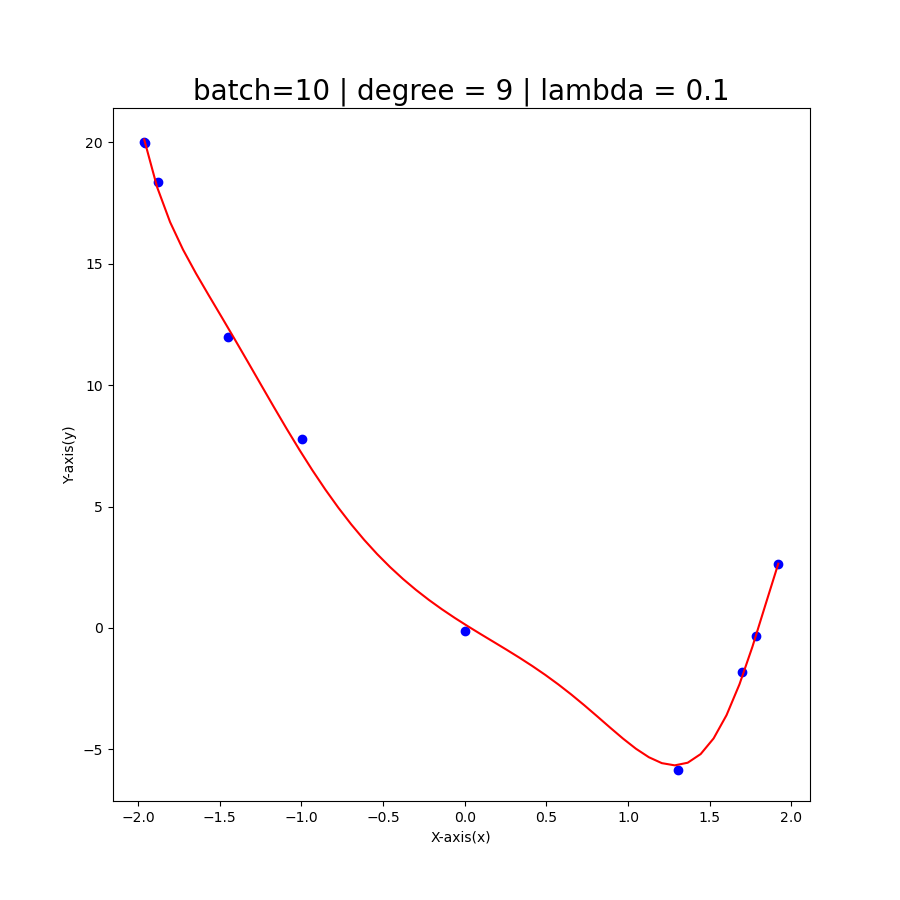
\includegraphics[width=.24\textwidth]{Task 1 Images/Batch 10/Figure_7.png}\hfill
    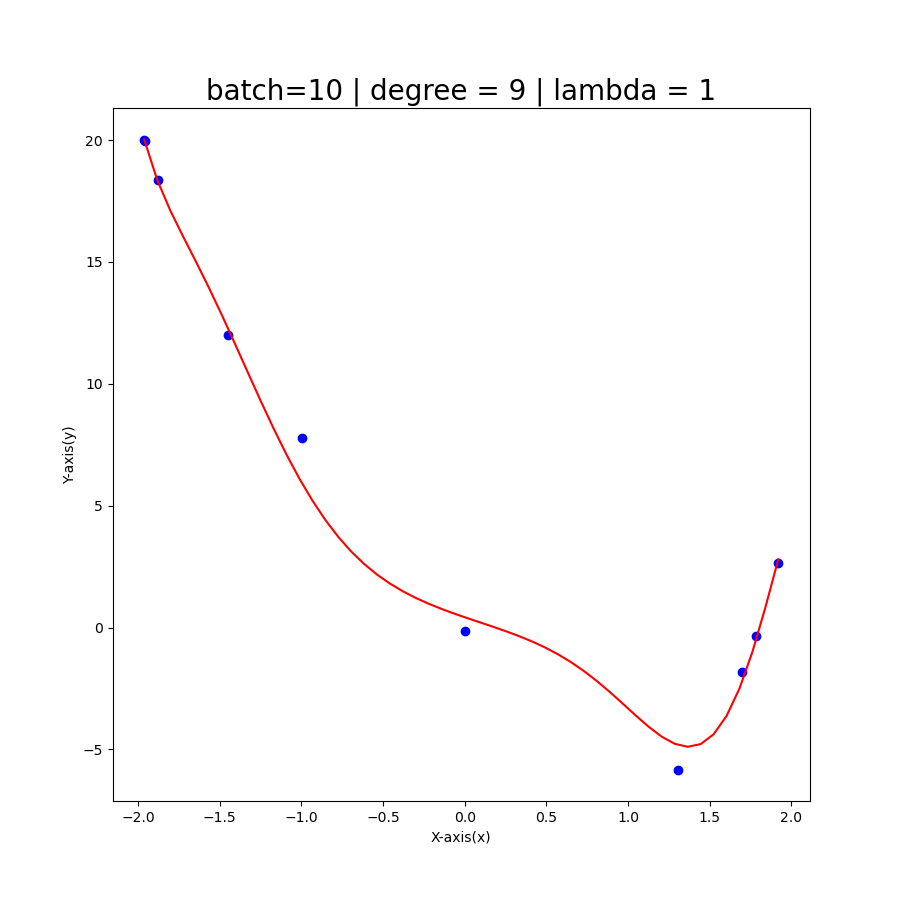
\includegraphics[width=.24\textwidth]{Task 1 Images/Batch 10/Figure_8.png}
    \caption{Plots of Polynomials having various orders of degree for a fixed regularisation parameter $\lambda = 1$ using 10 samples}
    \label{fig:2}
    \vspace*{\floatsep}

    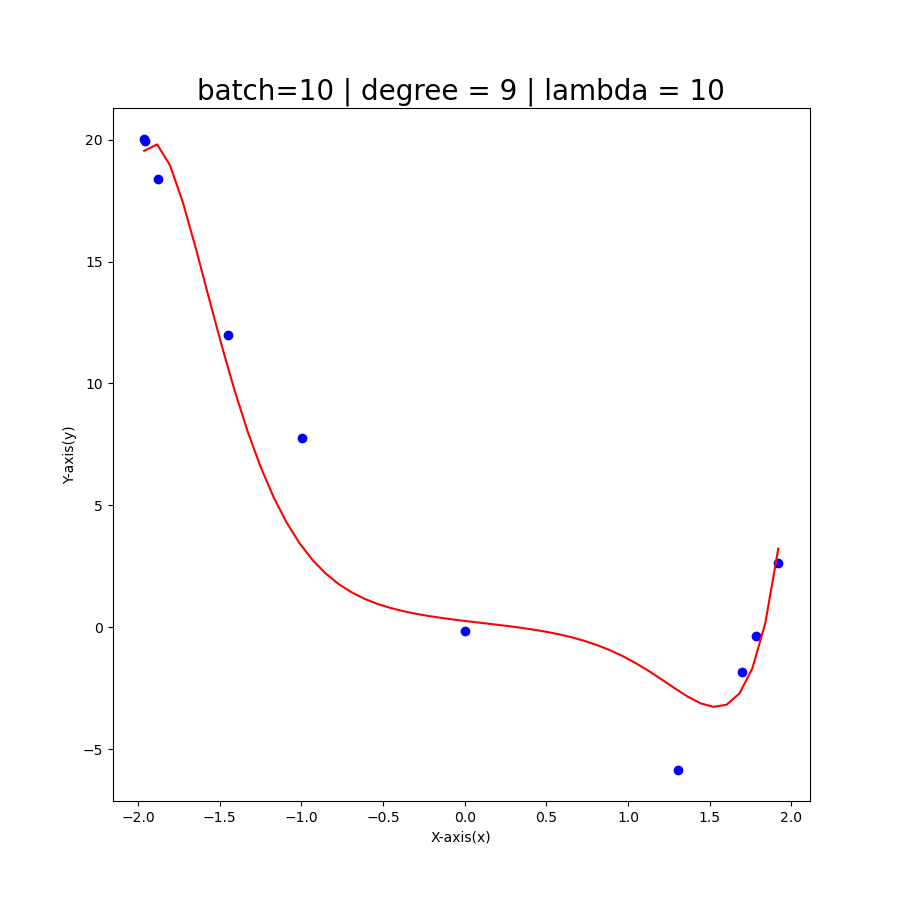
\includegraphics[width=.24\textwidth]{Task 1 Images/Batch 10/Figure_9.png}\hfill
    \includegraphics[width=.24\textwidth]{Task 1 Images/Batch 10/Figure_10.png}\hfill
    \includegraphics[width=.24\textwidth]{Task 1 Images/Batch 10/Figure_11.png}\hfill
    \includegraphics[width=.24\textwidth]{Task 1 Images/Batch 10/Figure_12.png}
    \caption{Plots of Polynomials having various orders of degree for a fixed regularisation parameter $\lambda = 0.1$ using 10 samples}
    \label{fig:3}
    \vspace*{\floatsep}

    \includegraphics[width=.24\textwidth]{Task 1 Images/Batch 10/Figure_13.png}\hfill
    \includegraphics[width=.24\textwidth]{Task 1 Images/Batch 10/Figure_14.png}\hfill
    \includegraphics[width=.24\textwidth]{Task 1 Images/Batch 10/Figure_15.png}\hfill
    \includegraphics[width=.24\textwidth]{Task 1 Images/Batch 10/Figure_16.png}
    \caption{Plots of Polynomials having various orders of degree for a fixed regularisation parameter $\lambda = 10$ using 10 samples}
    \label{fig:4}
\end{figure}    
    %\vspace*{\floatsep}
\begin{figure}[p]
    \includegraphics[width=.24\textwidth]{Task 1 Images/Batch 10/Figure 17.png}\hfill
    \includegraphics[width=.24\textwidth]{Task 1 Images/Batch 10/Figure 18.png}\hfill
    \includegraphics[width=.24\textwidth]{Task 1 Images/Batch 10/Figure 19.png}\hfill
    \includegraphics[width=.24\textwidth]{Task 1 Images/Batch 10/Figure 20.png}
    \caption{Plots of Polynomials having various orders of degree for a fixed regularisation parameter $\lambda = 1000$ using 10 samples}
    \label{fig:5}
    \vspace*{\floatsep}
    
    \includegraphics[width=.24\textwidth]{Task 1 Images/Batch 50/Figure 1.png}\hfill
    \includegraphics[width=.24\textwidth]{Task 1 Images/Batch 50/Figure 2.png}\hfill
    \includegraphics[width=.24\textwidth]{Task 1 Images/Batch 50/Figure 3.png}\hfill
    \includegraphics[width=.24\textwidth]{Task 1 Images/Batch 50/Figure 4.png}
    \caption{Plots of Polynomials having various orders of degree for a fixed regularisation parameter $\lambda = 0$ using 50 samples}
    \label{fig:6}
    \vspace*{\floatsep}
    
    \includegraphics[width=.24\textwidth]{Task 1 Images/Batch 50/Figure 5.png}\hfill
    \includegraphics[width=.24\textwidth]{Task 1 Images/Batch 50/Figure 6.png}\hfill
    \includegraphics[width=.24\textwidth]{Task 1 Images/Batch 50/Figure 7.png}\hfill
    \includegraphics[width=.24\textwidth]{Task 1 Images/Batch 50/Figure 8.png}
    \caption{Plots of Polynomials having various orders of degree for a fixed regularisation parameter $\lambda = 1$ using 50 samples}
    \label{fig:7}
    \vspace*{\floatsep}
    
    \includegraphics[width=.24\textwidth]{Task 1 Images/Batch 50/Figure 9.png}\hfill
    \includegraphics[width=.24\textwidth]{Task 1 Images/Batch 50/Figure 10.png}\hfill
    \includegraphics[width=.24\textwidth]{Task 1 Images/Batch 50/Figure 11.png}\hfill
    \includegraphics[width=.24\textwidth]{Task 1 Images/Batch 50/Figure 12.png}
    \caption{Plots of Polynomials having various orders of degree for a fixed regularisation parameter $\lambda = 0.1$ using 50 samples}
    \label{fig:8}
\end{figure}

\begin{figure}[p]
   \includegraphics[width=.24\textwidth]{Task 1 Images/Batch 50/Figure 13.png}\hfill
    \includegraphics[width=.24\textwidth]{Task 1 Images/Batch 50/Figure 14.png}\hfill
    \includegraphics[width=.24\textwidth]{Task 1 Images/Batch 50/Figure 15.png}\hfill
    \includegraphics[width=.24\textwidth]{Task 1 Images/Batch 50/Figure 16.png}
    \caption{Plots of Polynomials having various orders of degree for a fixed regularisation parameter $\lambda = 10$ using 50 samples}
    \label{fig:9}
    \vspace*{\floatsep}

    \includegraphics[width=.24\textwidth]{Task 1 Images/Batch 50/Figure 17.png}\hfill
    \includegraphics[width=.24\textwidth]{Task 1 Images/Batch 50/Figure 18.png}\hfill
    \includegraphics[width=.24\textwidth]{Task 1 Images/Batch 50/Figure 19.png}\hfill
    \includegraphics[width=.24\textwidth]{Task 1 Images/Batch 50/Figure_20.png}
    \caption{Plots of Polynomials having various orders of degree for a fixed regularisation parameter $\lambda = 1000$ using 50 samples}
    \label{fig:10}
    \vspace*{\floatsep}
\end{figure}
\newpage
\begin{figure}[b]
    \centering
    \begin{subfigure}[t]{0.25\textwidth}
        \centering
        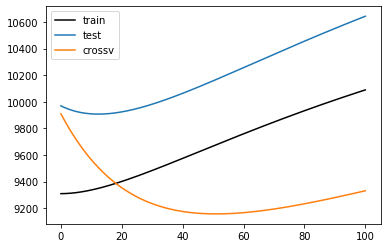
\includegraphics[height=1in]{Task 2 Images/batch500_deg2_lambda.png}
        \caption{Degree, $M = 2$}
    \end{subfigure}%
    ~ 
    \begin{subfigure}[t]{0.25\textwidth}
        \centering
        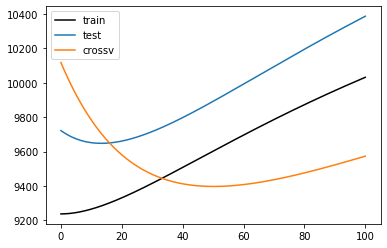
\includegraphics[height=1in]{Task 2 Images/batch500_deg3_lambda.png}
        \caption{Degree, $M = 3$ }
    \end{subfigure}%
    ~
    \begin{subfigure}[t]{0.25\textwidth}
        \centering
        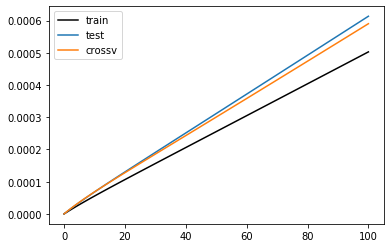
\includegraphics[height=1in]{Task 2 Images/batch500_deg6_lambda1to100.png}
        \caption{ Degree, $M = 6$}
    \end{subfigure}
    \caption{Effect of $\lambda$}
    \label{fig:11}
\end{figure}

\begin{figure}[p]
    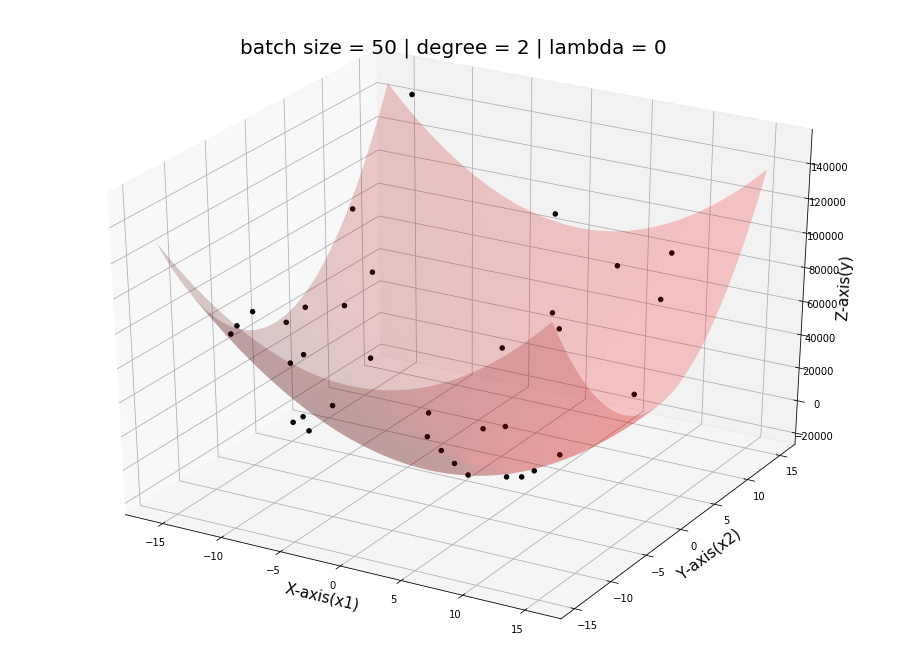
\includegraphics[width=.30\textwidth]{Task 2 Images/surfaceplot_batch50_deg2_lamb0.png}\hfill
    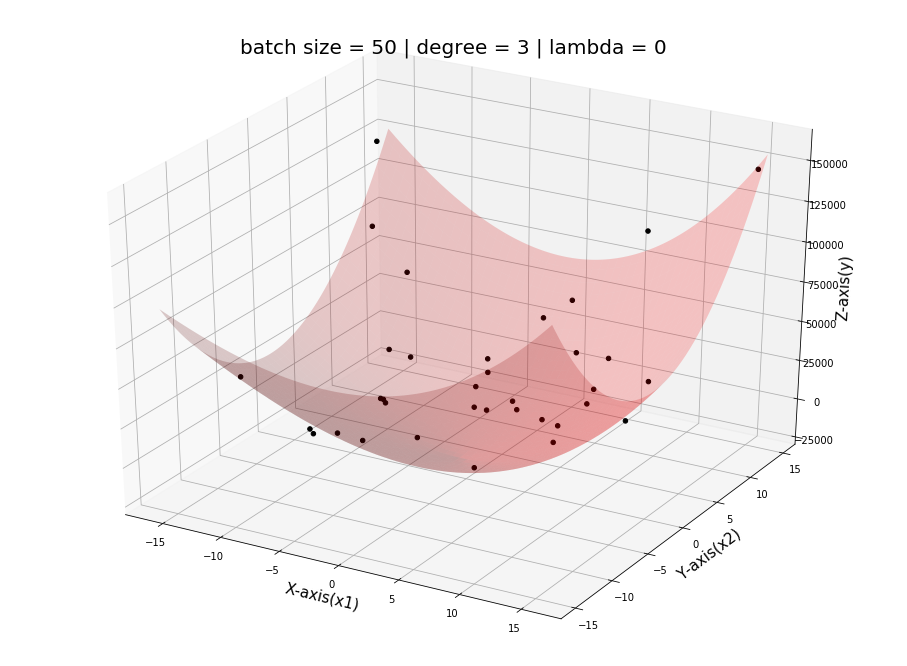
\includegraphics[width=.30\textwidth]{Task 2 Images/surfaceplot_batch50_deg3_lamb0.png}\hfill
    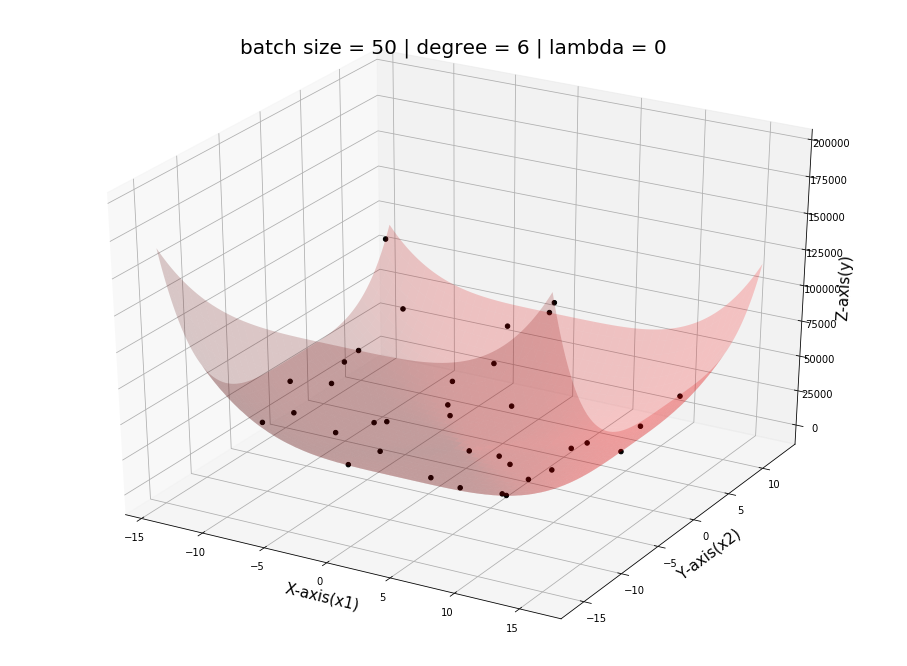
\includegraphics[width=.30\textwidth]{Task 2 Images/surfaceplot_batch50_deg6_lamb0.png}
    \caption{Surface Plots using various degree for a fixed best regularisation parameter $\lambda = 0$ using 50 samples }
    \label{fig:12}
    \vspace*{\floatsep}
    
    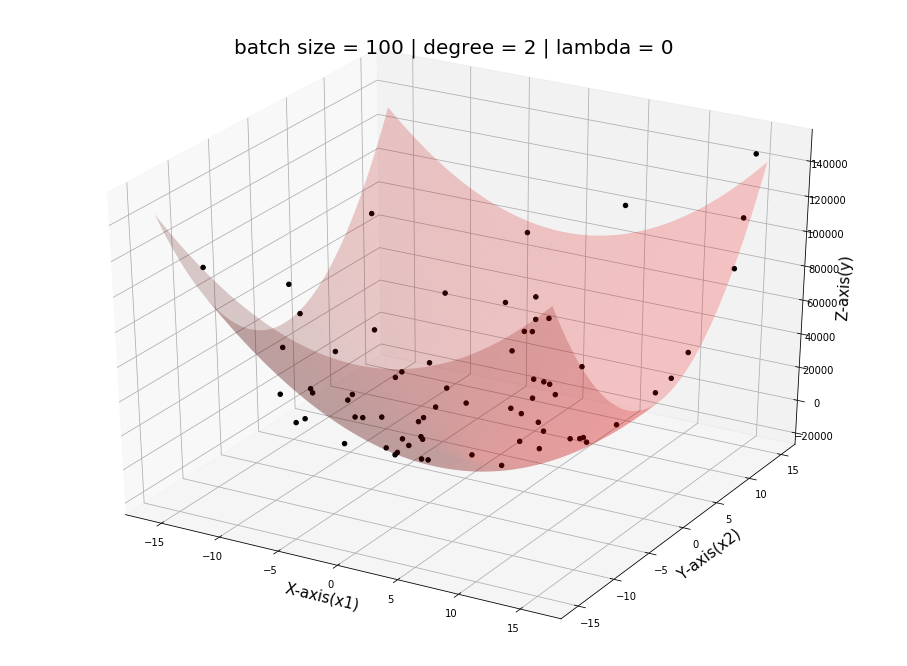
\includegraphics[width=.30\textwidth]{Task 2 Images/surfaceplot_batch100_deg2_lamb0.png}\hfill
    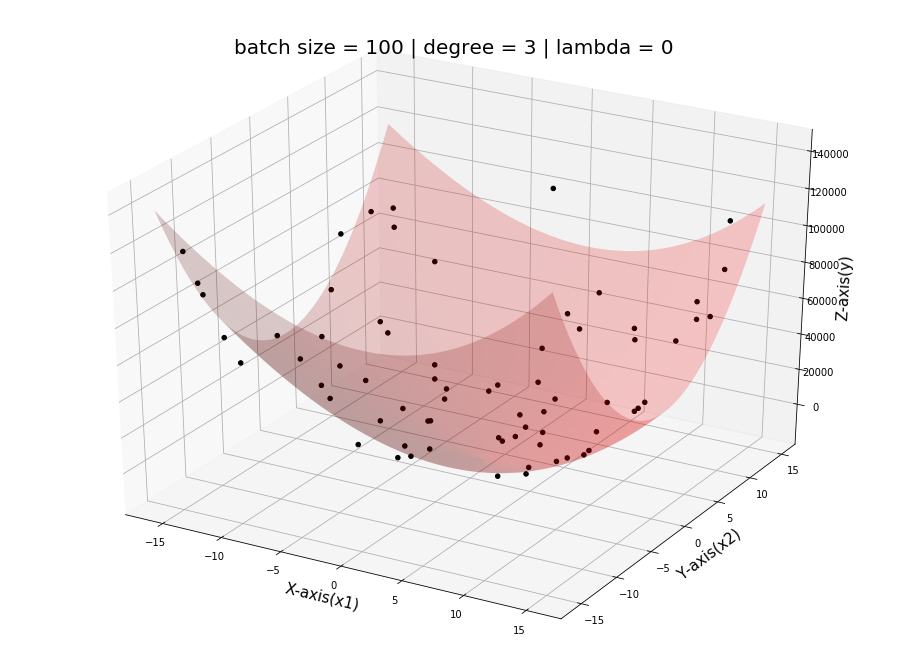
\includegraphics[width=.30\textwidth]{Task 2 Images/surfaceplot_batch100_deg3_lamb0.png}\hfill
    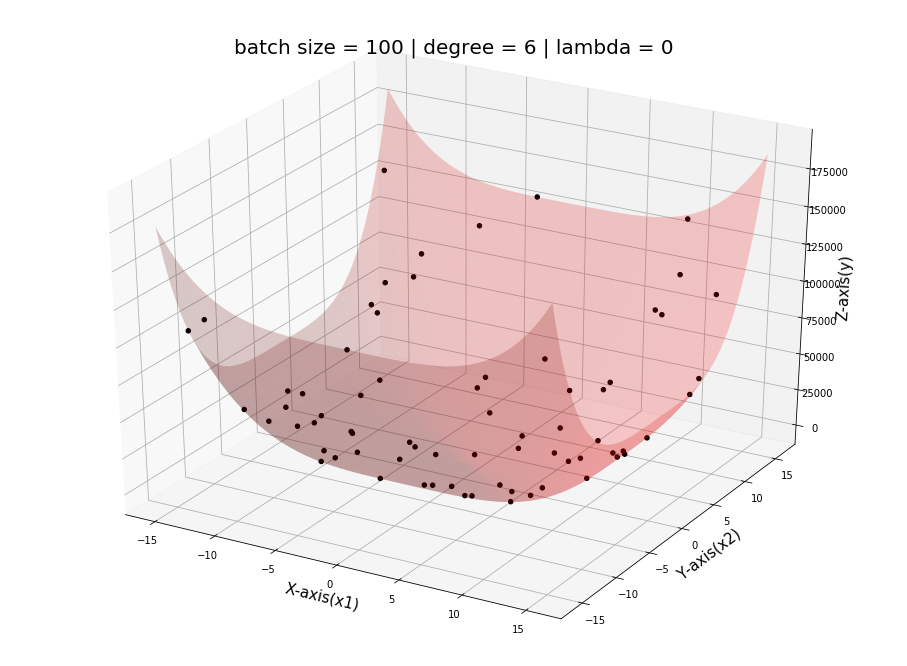
\includegraphics[width=.30\textwidth]{Task 2 Images/surfaceplot_batch100_deg6_lamb0.png}
    \caption{Surface Plots using various degree for a fixed regularisation parameter $\lambda = 0$ using 100 samples}
    \label{fig:13}
    \vspace*{\floatsep}
    
    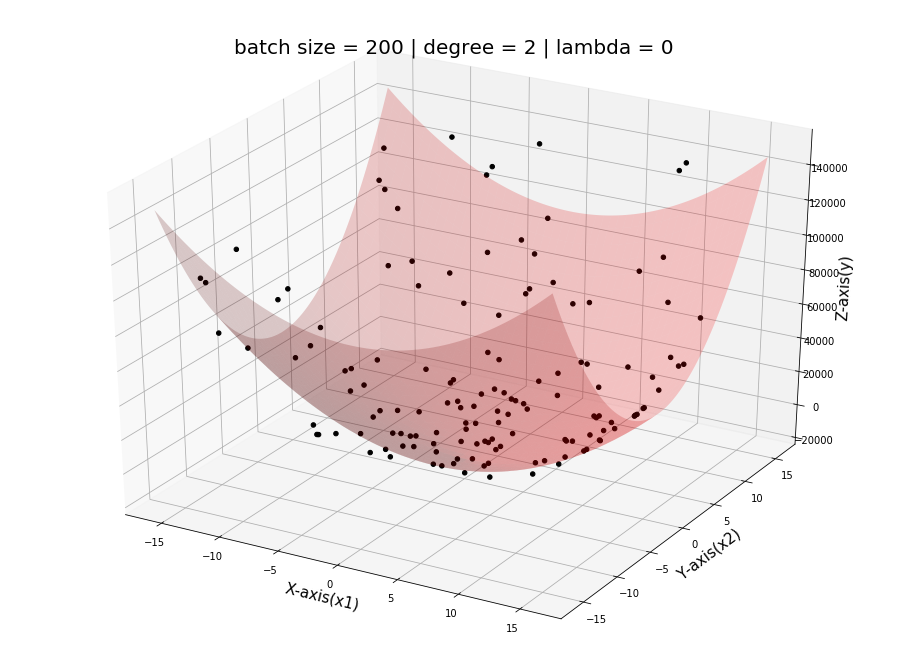
\includegraphics[width=.30\textwidth]{Task 2 Images/surfaceplot_batch200_deg2_lamb0.png}\hfill
    \includegraphics[width=.30\textwidth]{Task 2 Images/surfaceplot_batch200_deg2_lamb0.png}\hfill
    \includegraphics[width=.30\textwidth]{Task 2 Images/surfaceplot_batch200_deg2_lamb0.png}
    \caption{Surface Plots using various degree for a fixed regularisation parameter $\lambda = 0$ using 200 samples}
    \label{fig:14}
    \vspace*{\floatsep}
    
    \includegraphics[width=.30\textwidth]{Task 2 Images/surfaceplot_batch500_deg2_lamb0.png}\hfill
    \includegraphics[width=.30\textwidth]{Task 2 Images/surfaceplot_batch500_deg3_lamb0.png}\hfill
    \includegraphics[width=.30\textwidth]{Task 2 Images/surfaceplot_batch500_deg6_lamb0.png}
    \caption{Surface Plots using various degree for a fixed regularisation parameter $\lambda = 0$ using 500 samples}
    \label{fig:15}
\end{figure}

\begin{figure}[tb]
     \centering
     \begin{subfigure}[t]{0.30\textwidth}
         \centering
         \includegraphics[height=1.6in]{Task 2 Images/best_scatterplot_batch_500_degree_6_lambda_0_training.png}
         \caption{Training Data}
     \end{subfigure}%
     ~ 
     \begin{subfigure}[t]{0.30\textwidth}
         \centering
         \includegraphics[height=1.6in]{Task 2 Images/best_scatterplot_batch_500_degree_6_lambda_0_test.png}
         \caption{Test Data }
     \end{subfigure}%
     ~
     \begin{subfigure}[t]{0.30\textwidth}
         \centering
         \includegraphics[height=1.6in]{Task 2 Images/best_scatterplot_batch_500_degree_6_lambda_0_validation.png}
         \caption{Validation Data }
     \end{subfigure}
     \caption{Best Scatter Plot}
     \label{fig:16}
\end{figure}
\newpage
\begin{figure}[t]
    \centering
    \begin{subfigure}[t]{0.50\textwidth}
        \centering
        \includegraphics[height=1.6in]{Task 3 Images/3.1.42.png}
        \caption{Training Data}
    \end{subfigure}%
    ~ 
    \begin{subfigure}[t]{0.50\textwidth}
        \centering
        \includegraphics[height=1.6in]{Task 3 Images/3.1.41.png}
        \caption{Test Data }
    \end{subfigure}%
    \caption{Scatter Plot of the Gaussian Basis Function of the best performing model for Dataset 2}
    \label{fig:17}
\end{figure}

\begin{figure}[tb]
    \centering
    \begin{subfigure}[t]{0.50\textwidth}
        \centering
        \includegraphics[height=1.6in]{Task 3 Images/3.2.51.png}
        \caption{Training Data}
    \end{subfigure}%
    ~ 
    \begin{subfigure}[t]{0.50\textwidth}
        \centering
        \includegraphics[height=1.6in]{Task 3 Images/3.2.52.png}
        \caption{Test Data }
    \end{subfigure}%
    \caption{Scatter Plot of the Gaussian Basis Function of the best performing model for Dataset 3}
    \label{fig:18}
\end{figure}
